\chapter{\label{CH:Pipeline}TuMag's pipeline and data.}


The 2024 observational campaign of the third edition of the Sunrise observatory took place beetween the 11$^{\text{th}}$ and 17$^{\text{th}}$ of July and was a success. In contrast to previous flights, where technical challenges limited the number of useful observations, all subsystems performed well during this third flight, allowing for nearly continuous instrument operation over more than six days. From TuMag’s perspective, the campaign yielded approximately 10 terabytes of data, consisting of over 40 scientific observation blocks and 250 calibration observations.

The substantial volume of data generation by the three instruments, requires that the data must be physically recovered on-site after flight termination, since they cannot be broadcasted from the observatory to the operations center. Recovery activities began immediately after landing and lasted until early August, during which all surviving components, along with the data vaults, were transported to Yellowknife, Canada, the nearest city to the landing site. The data vaults arrived at MPS in early August, where a backup was created before the data associated with each instrument was sent to the respective PI institution. TuMag’s data arrived at  IAA in late August, marking the official start of the reduction process.

The reduction process began by labeling all images and identifying the more than 600 thousand images captured by TuMag. Once the observations were correctly identified, the reduction process commenced and, at the time of writing, remains ongoing. Due to the relevance of the pipeline development and results for this thesis, this chapter will provide an overview of TuMag's data and the current state of its pipeline, although the results remain preliminary.

The discussion will begin by introducing TuMag’s various observing modes, both scientific and calibration, followed by a brief review of the observation campaign, outlining the different observation programs and their scientific objectives. The chapter will conclude with an examination of the data reduction process, detailing the pipeline and presenting some initial results. It is important to note that, due to the late arrival of the data, this thesis had to be written in parallel with the reduction process. Therefore, the results presented here are preliminary, and the final product will differ as additional reduction steps are incorporated.

\section{TuMag's observing modes}

With the purpose of simplifying the operations activities, TuMag operates through a series of so-called observing modes. The observing modes are a list of pre-configured settings tailored for various observations, including both calibration and scientific purposes. Each mode is designed to fulfill the specific objectives of the corresponding observation and enables nearly automatic operation of the instrument during flight.

\begin{table}
    \centering
   \begin{tabular}{cccccccc}
    \hline
    \hline
    Observing mode & Spectral lines  & $N_\lambda$ & $N_P$ & $N_a$& $N_c$ & $t_{\text{eff}} (s)$ & (S/N) \\
    \hline
    0s & Mg I $b_2$ 5172.7 \r{A} & 12 & 1 & 2 & 1 & 6.3 & 500\\ 
    0p & Mg I $b_2$ 5172.7 \r{A} & 12 & 4 & 16 & 1 & 37.62 & 1000\\
    1  & Mg I $b_2$ 5172.7 \r{A} &  10 & 4 & 16 & 1 & 31.81 & 1000\\
    2  & Fe I 5250.2 \r{A}, Fe I 5250.6 \r{A} &  8 & 4 & 16 & 1 & 23.4 & 1000\\
    3  & Fe I 5250.2 \r{A}, Fe I 5250.6 \r{A} & 5 & 2 & 20 & 1 & 10.04 & 1000\\
    4  & Mg I $b_2$ 5172.7 \r{A} & 3 & 4 & 10 & 10 & 54.01 & 2500\\
    5  & Fe I 5250.2 \r{A}, Fe I 5250.6 \r{A} & 3 & 4 & 10 & 10 & 53.60 & 2500\\ 
    \hline
    \hline
    \end{tabular}
    \caption{Scientific observing modes. From left to right, the columns are: observing mode identicator, measured spectral lines, number of wavelengths, number of modulations, number of accumulations, number of cycles, the effective exposure time and the polarimetric S/N.}
    \label{table: scientific observing modes}
\end{table}

A summary of the properties for each observing mode is provided in Table \ref{table: scientific observing modes}. There are four distinct modes designed to observe the magnesium line. Mode 0s performs a fast, extended scan of the spectral line using 12 wavelength samples: [-40, -30, -20, -10, 0, 10, 20, 30, 40, 50, 60, 65] pm\footnote{Sampling positions are given relative to the line core.}, with two accumulations ($N_a = 2$) to maximize scanning speed, and no modulation ($N_P = 1$). Mode 0p is similar to mode 0s but employs a full-vector modulation scheme, $N_P = 4$, requiring $N_a = 16$ to ensure the required S/N. Mode 1 provides a shortened scan of the magnesium line, with measurements taken at [-30, -20, -10, -5, 0, 5, 10, 20, 30, 65] pm, also utilizing the same full-vector modulation scheme. Finally, mode 4 is a "deep" magnetic mode, featuring a highly reduced scan with only three samples at [-10, 0, 10] pm, but with $N_a = 10$ and $N_c = 10$ cycles, the latter forcing a repetition of the modulation cycle, thus enhancing the polarimetric sensitivity by increasing the effective exposure time for each modulation and wavelength.

Three observing modes are configured for the iron lines. Mode 2 employs a vectorial modulation scheme applicable to both iron lines, with sampling at [-12, -8, -4, 0, 4, 8, 12, 22] pm. Mode 3 uses a longitudinal modulation scheme, measuring only Stokes I and V, with samples taken at [-8, -4, 4, 8, 22] pm. Lastly, mode 5 closely resembles mode 4, but is configured for the iron lines, with sampling at [-8, 0, 8] pm. The only difference between these two modes is the wavelength sampling scheme.

Although most of the parameters are set up by the observing mode and cannot be changed, there are some configurable parameters that allow to slightly modify the observing modes to fit the specific goal of the observation. The most important among these are the following:

\begin{itemize}
    \Myitem $\lambda _ {\text{rep}}$ : A parameter that allows to repeat all the observations carried out at every spectral position before changing wavelength. This parameter is employed for flat-field observations (see the following section) or enhancing the S/N of a specific observation. By default is set to 1.
    \Myitem Etalon offset : A parameter that allows for the introduction of a global shift to the spectral sampling by offsetting the absolute voltages of the scan, and thus, the wavelengths. This parameter was used to center the spectral line in shorter observing modes affected by solar rotation or other effects that might shift the spectral position. The default value is set to 0 V.
    \Myitem $N_a$ : Even though the number of accumulations is fixed in nominal observing modes, this parameter was set as configurable in order to allow modifications for faster observations when needed. The  default value depends on the observing mode.  
\end{itemize}

\begin{figure}[t]
    \begin{minipage}[c]{0.67\textwidth}
      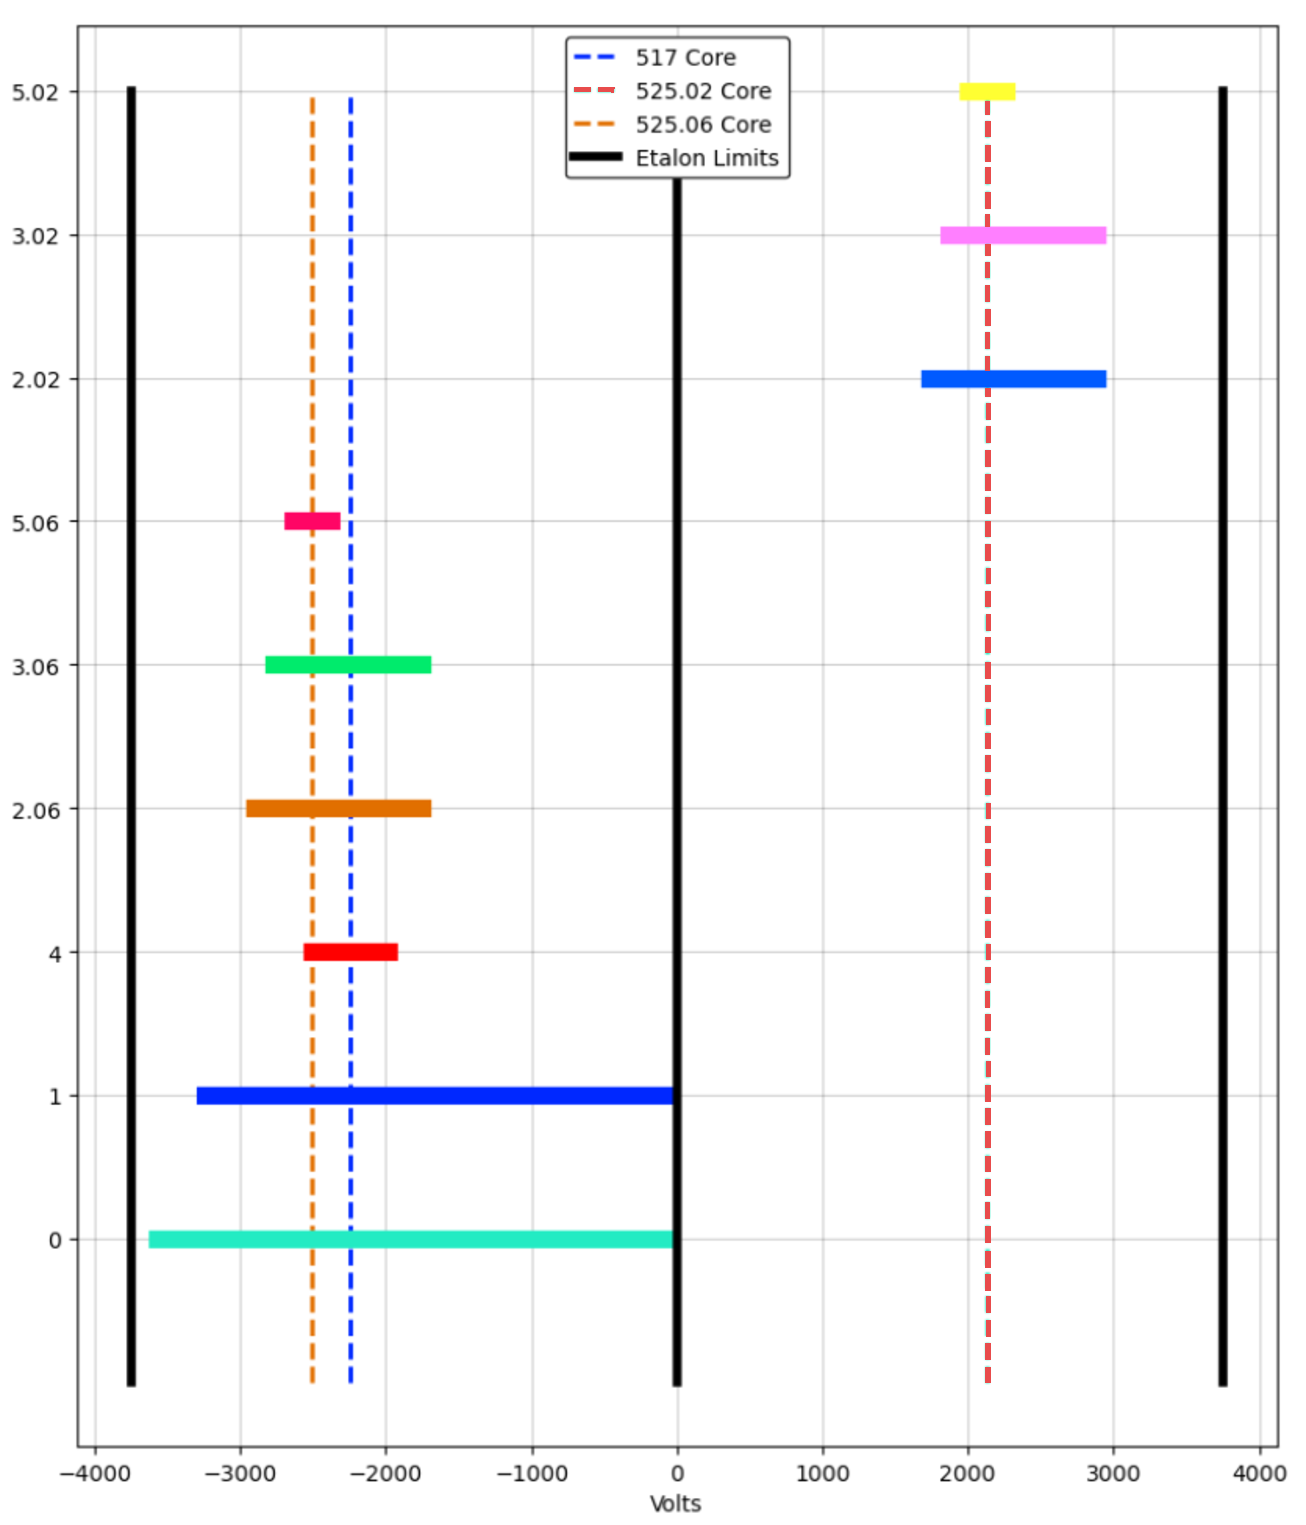
\includegraphics[width=\textwidth]{figures/Pipeline/obs_modes.pdf}
    \end{minipage}\hfill
    \begin{minipage}[c]{0.29\textwidth}
      \caption[Voltage ranges of TuMag's observation modes.]{
       Schematic representation of the voltage range covered by all observing modes. The dashed lines indicate the position of the line core as measured during the E2E tests performed at INTA in December 2021. The black vertical lines represent the voltage limits that cannot be crossed in an observing mode. The colored horizontal lines represent the voltage range covered by the observing modes, each represented in a different color and labeled on the left.  
       \label{fig_pipeline: Observing modes ranges}} 
    \end{minipage}
\end{figure}

Figure \ref{fig_pipeline: Observing modes ranges} presents a schematic representation of the voltage ranges for the observing modes when converting spectral sampling to volts. The black lines indicate the voltage boundaries that cannot be surpassed during an observation due to technical constraints. These limits are set at $\pm 3750$ V as the maximum and minimum values, with an additional limitation at 0 V, since a polarity change poses technical challenges that could not be addressed during an observation mode. These restrictions are important for two cases: first, for magnesium observation modes, specifically modes 1 and 0, where the continuum measurement is positioned as far from the core as possible, at -80 V, due to the 0 V crossing limitation. Second, when applying an etalon offset to shift the spectral positions of a particular observing mode as the offset cannot cause the final positions to exceed these boundaries.

\subsection{Calibration modes}
An additional type of observing modes are also designed for carrying out calibration observations. These calibration observing modes are more flexible than nominal ones, and allow for the configuration of several parameters to better match the observations.

\begin{figure}[t]
    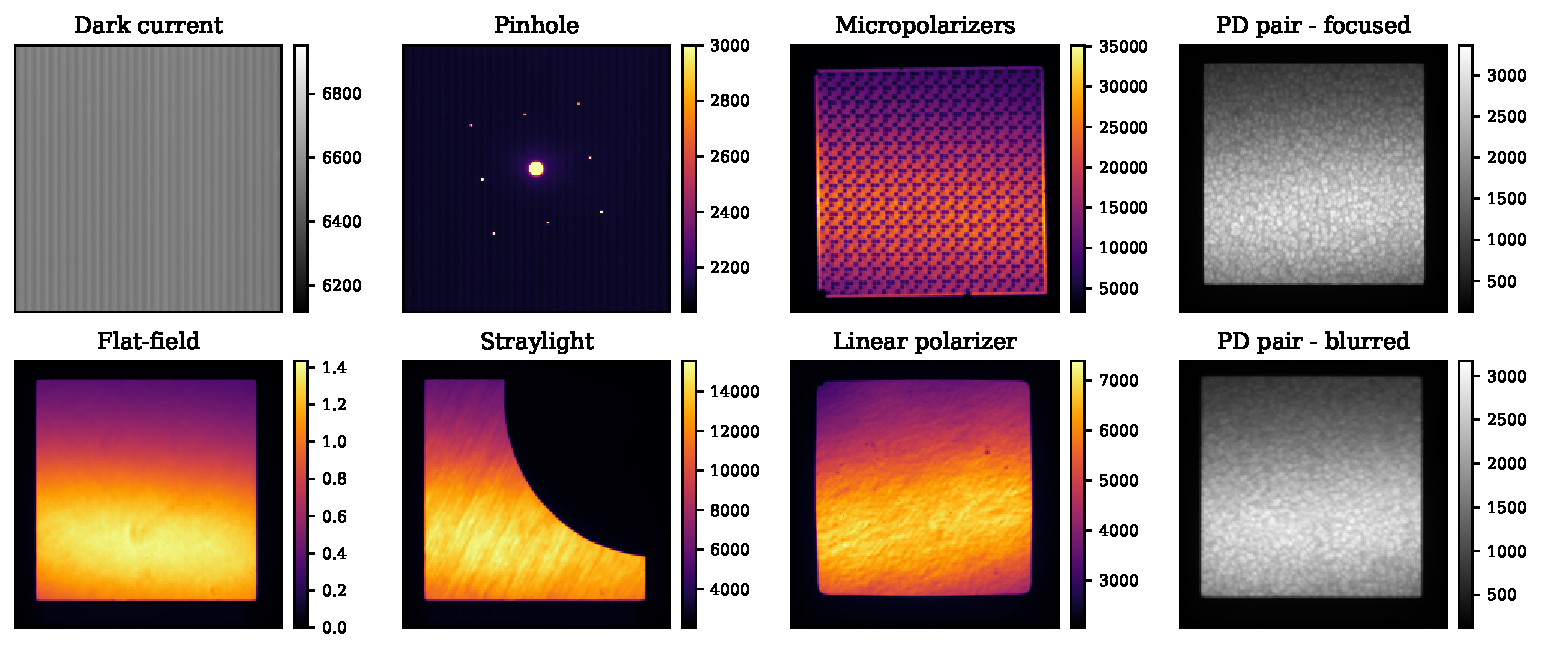
\includegraphics[width=\textwidth]{figures/Pipeline/cal_modes_examples.pdf}
    \caption[Calibration observation modes examples of TuMag.]{
      Examples of calibration observations. All images, with the exception of the flat-field, are presented in their raw format, without any manipulation or correction applied. The flat-field observation depicted corresponds to the first modulation of the continuum measurement obtained during a flat-field observation corresponding to observing mode 1. All data belong to camera 1, and the colorbar is calibrated in digital counts except for the flat-field which is normalized to its mean value. }
      \label{fig_pipeline: cal_examples}
\end{figure}

\subsubsection{Flat-field observations}

One of the essential calibration procedures in any telescope-based astronomical observation is the acquisition of flat-field images. These observations are designed to measure intensity variations across the FoV, which arise from several factors, including dust particles, pixel efficiency variations, or in TuMag's case, intensity gradients induced by the etalon, among other sources. The aim is to produce an observation with a uniformly flat intensity distribution. However, achieving such flat-field observations is not always straightforward, particularly for certain instruments. While night-time telescopes can utilize twilight periods to observe areas of the sky devoid of stars, solar telescopes, such as Sunrise III, must look for alternative methods. 

In Sunrise III, flat-field images are generated by deliberately blurring the solar scene through rapid movements of the telescope itself. This is done by the pointing system of the gondola, which allows for moving the FoV in a particular path with the goal of mixing as much as possible the solar granulation. In the end, this process effectively removes the solar structure from the FoV when averaging out multiple blurred observations, resulting in a flat-field image devoid of solar features.

In the case of TuMag, flat-field observations are performed using a modified version of each nominal observing modes, where the $\lambda_{\text{rep}}$ is set to 4. Additionally, multiple consecutive instances ($N_{\text{reps}}$) of these observations are executed, typically 5 or 7. During data processing, a single flat-field is generated for each wavelength and modulation state by averaging all corresponding observations. Finally, the flats are normalized, typically, to a central area, one by one in order to remove the spectral line features from the flats.

Figure \ref{fig_pipeline: cal_examples} shows an example of a flat-field observation, for one camera, modulation and wavelength (bottom left panel). The image shows a clear deviation from flatness in the measurement, primarily due to the etalon intensity gradient, which accounts for the change in intensity between the brighter bottom half and the darker top half, and some minor inhomogeneities over the FoV. 

\subsubsection{Dark-current observations}

A second critical calibration procedure for any observation involving electronic cameras is the measurement of the dark current. In the absence of incident photons, electrons within the camera wells can still be randomly excited. This spontaneous excitation can be incorrectly interpreted as photon-induced counts when analyzing the data. Dark current observations are designed to characterize these random electronic excitations, which are primarily influenced by the camera physical conditions, particularly temperature, so that they can be accurately subtracted from the final images. In the case of TuMag, the camera, hereafter SPGCam,  is based on the rolling shutter, backside-illuminated GPIXEL SENSE GSENSE400BSI 2 k x 2 k pixel detector \citep{tumag-cams}. The dark current of the SPGCam, also used for SCIP, is dominated by several sources of error since the camera is used in ambient temperature. In particular, besides the photon noise and the typical termal dark current, the sensor also shows a dominant fixed pattern noise characterized by sequential vertical strips which needs to be removed in the observations.  

For TuMag, dark current calibration involved capturing a series of 50 images with $N_a = 50$ with no light entering the instrument. As with flat-field observations, a single dark current frame for each camera is generated by averaging all individual observations. In the top left panel of Fig. \ref{fig_pipeline: cal_examples} a dark current shot is depicted, characterized by the vertical strips of the fixed pattern noise.  

\subsubsection{Linear polarizer and micropolarizers observations.}

TuMag's filter wheels are equipped with two targets designed to assess the instrument polarimetric performance: a linear polarizer and a set of micropolarizers. Both targets are situated in the first filter wheel and are used in conjunction with the three distinct prefilters located in the second filter wheel. The linear polarizer serves to evaluate the polarimetric calibration, particularly by quantifying the level of cross-talk betweeen Stokes Q, U, and V, as no circular polarization should be detected when using this target. The micropolarizers provide a more complete assessment, as they consist of multiple linear polarizers oriented at different angles. 

Observations with these targets are carried with the three prefilters, at a single wavelength, located in the continuum of each line. For each measurement, a vectorial modulation scheme is employed that allows for the derivation of the four Stokes parameters. In the third column of figure \ref{fig_pipeline: cal_examples} observations of both targets are shown. 

\subsubsection{Pinhole Observations.}

Another calibration target included in the filter wheels is the pinhole target. This target blocks most of the light reaching the instrument, except for a few small holes arranged in a square-like pattern across the FoV, as shown in the top panel of the second column of figure \ref{fig_pipeline: cal_examples}. A larger hole is located at the center of the FoV, surrounded by eight smaller holes that trace a square with the central hole at its midpoint. These observations serve various purposes, including image alignment, detecting the presence of ghost images, identifying etalon reflections, and determining the PSF of the instrument.

Pinhole observations are conducted similarly to those with polarizers, that is, in combination with the three prefilters at a single wavelength (the continuum of each line), but without applying any modulation.

\subsubsection{Stray-light target.}

Not all the light that reaches the detector is necessarily the intended signal for a given observation. Some unwanted light, primarily originating from internal reflections along the optical path, may also reach the instrument. This unwanted contribution, known as stray-light, contaminates the measurements by reducing contrast, lowering the S/N, and generally degrading the spectral, optical, and polarimetric performance of the instrument.

To address this contamination, TuMag performed a series of observations using a target that blocks part of the FoV (see the bottom panel of the second column of figure \ref{fig_pipeline: cal_examples}). By analyzing the dark region in these observations, it becomes possible to measure and model the stray-light reaching the instrument, allowing for its subsequent removal from the data.

\subsubsection{\label{ref:spectral_scans}Pre-filter scans.}

TuMag observations are very sensitive to spectral shifts either from the pre-filters or from the observed spectral line position. The shift of the pre-filters can happen due to changes in the physical conditions of the filter wheels, mainly temperature, which spectrally shift their transmission peak. The position of their transmission peak affects the measurements: the further we are from the peak transmission the less the signal to noise due to the decreased transmission, as observed from the decreasing gradient in tranmsission as wavelengths increase in distance to the line core. Aditionally, even though the temperature of the filter wheels is controlled at all times, small changes in temperature could affect the pre-filter bandpass which can allow for transmission of secondary orders of the etalon to contaminate the measurement.

Furthermore, due to solar rotation, the spectral position at which the spectral lines are recorded can change. This effect is specially important in observing modes that require great spectral accuracy, such as the deep modes, where only three spectral positions close to the line core are employed. Although this effect is unavoidable and generally of second order, knowing beforehand the position at which a spectral line is recorded allow us to account for this shift in observations that are specially sensible.  

To verify the behavior of the pre-filters, quantify the contribution from the etalon secondary orders, and measure the position of spectral lines, TuMag performs the so-called pre-filter scans, typically conducted before and after observations. These scans involve a rich spectral sweep using the pre-filters employed during the observations, capturing the voltage range of each specific line at intervals of 100 V without modulating. Figure \ref{fig_pipeline: prefilter_scans} presents an example of these scans for each pre-filter, recorded during the commissioning phase of the observation campaign. In section \ref{sect:pipeline_prefilter_scans_fit} we detail how these observations are utilized and provide a brief discussion of the results.


\begin{figure}[t]
    \begin{minipage}[c]{0.67\textwidth}
      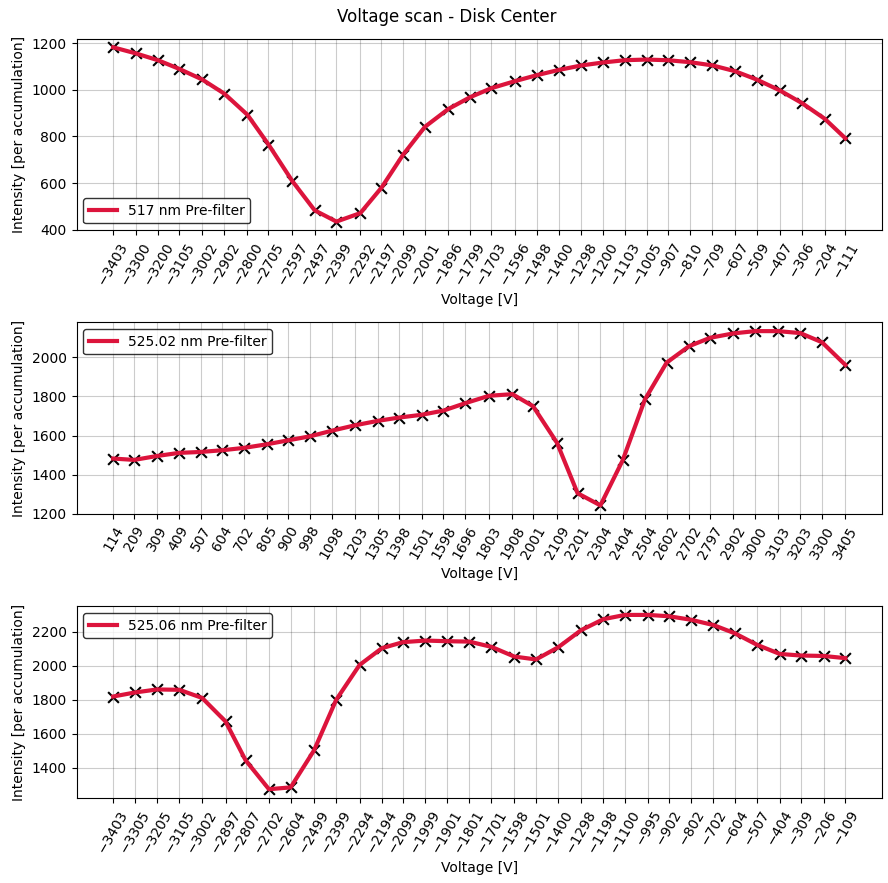
\includegraphics[width=\textwidth]{figures/Pipeline/Prefilter_scans.png}
    \end{minipage}\hfill
    \begin{minipage}[c]{0.29\textwidth}
      \caption[Average intensities measured for each pre-filter.]{
       Average intensities per accumulation in the center of the FoV of the pre-filter scans performed during the commissioning of the instruments during the first hours of the Sunrise III 2025 campaign.  
       \label{fig_pipeline:  prefilter_scans}
      } 
    \end{minipage}
  \end{figure}


\subsubsection{\label{susec: PD_measurements}Phase diversity}

Lastly, TuMag is equipped with the capability to perform phase diversity for image reconstruction. As discussed in previous chapters, applying image reconstruction techniques is essential to meet the optical quality requirements. To this end, TuMag includes a PD plate in the first filter wheel that introduces a known defocus in the images. Capturing images with and without this plate enables the computation of the instrument's spatial PSF, which can then be deconvolved from the data.

PD measurements require quasi-simultaneous pairs of aberrated and unaberrated images. Therefore, TuMag's PD observations consist of a series of 40 rapid, non-accumulated frames with the PD plate, followed by a corresponding series without the PD plate. The feasibility of this sequential scheme for phase diversity techniques has been confirmed in \cite{PD_sequential}. A pair of focused-defocused images of quiet-Sun observations is shown in the last column of Figure \ref{fig_pipeline: cal_examples}.

\section{Timelines}

The operations of Sunrise III were designed to be nearly autonomous to ensure synchronization between the scientific instruments, the telescope, and the CWS, and limit issues in case of a problem with communication for sending telecommands. Given the limited time available for the observation campaign, this autonomy also helps to speed up operations, enabling more observation programs to be accommodated within the mission duration.

The Sun is a highly dynamic system, exhibiting a wide range of behaviors and phenomena, from large-scale structures such as active regions, or pores, which harbor strong magnetic fields, to smaller, quiet Sun areas containing the so-called network and intranetwork fields, where the solar gas mostly drives the dynamics and structuring of the magnetic fields. This diversity, observable in various spectral ranges and across different regions of the solar disk, demands multiple observations with distinct characteristics.

Prior to the first flight of Sunrise III in 2022, a series of timelines were developed to program both calibration and scientific observation blocks. These timelines were carefully designed by the Sunrise Science Team, taking into account the 70 observing proposals submitted for Sunrise.

Observing proposals that could be fulfilled by targeting the same solar feature, while considering its disk position, were grouped into a single timeline. Each timeline included not only the necessary scientific observation blocks but also the required calibration observations to ensure data accuracy. Thus, timelines consist of a sequence of scientific and calibration observation blocks. The observing blocks within a timeline could vary in content depending on the scientific objectives and the status of the other instruments involved.

In the case of TuMag, each observing block was composed either of a combination of two observing modes executed consecutively, or a single observing mode repeated throughout the block.  

\begin{figure}
  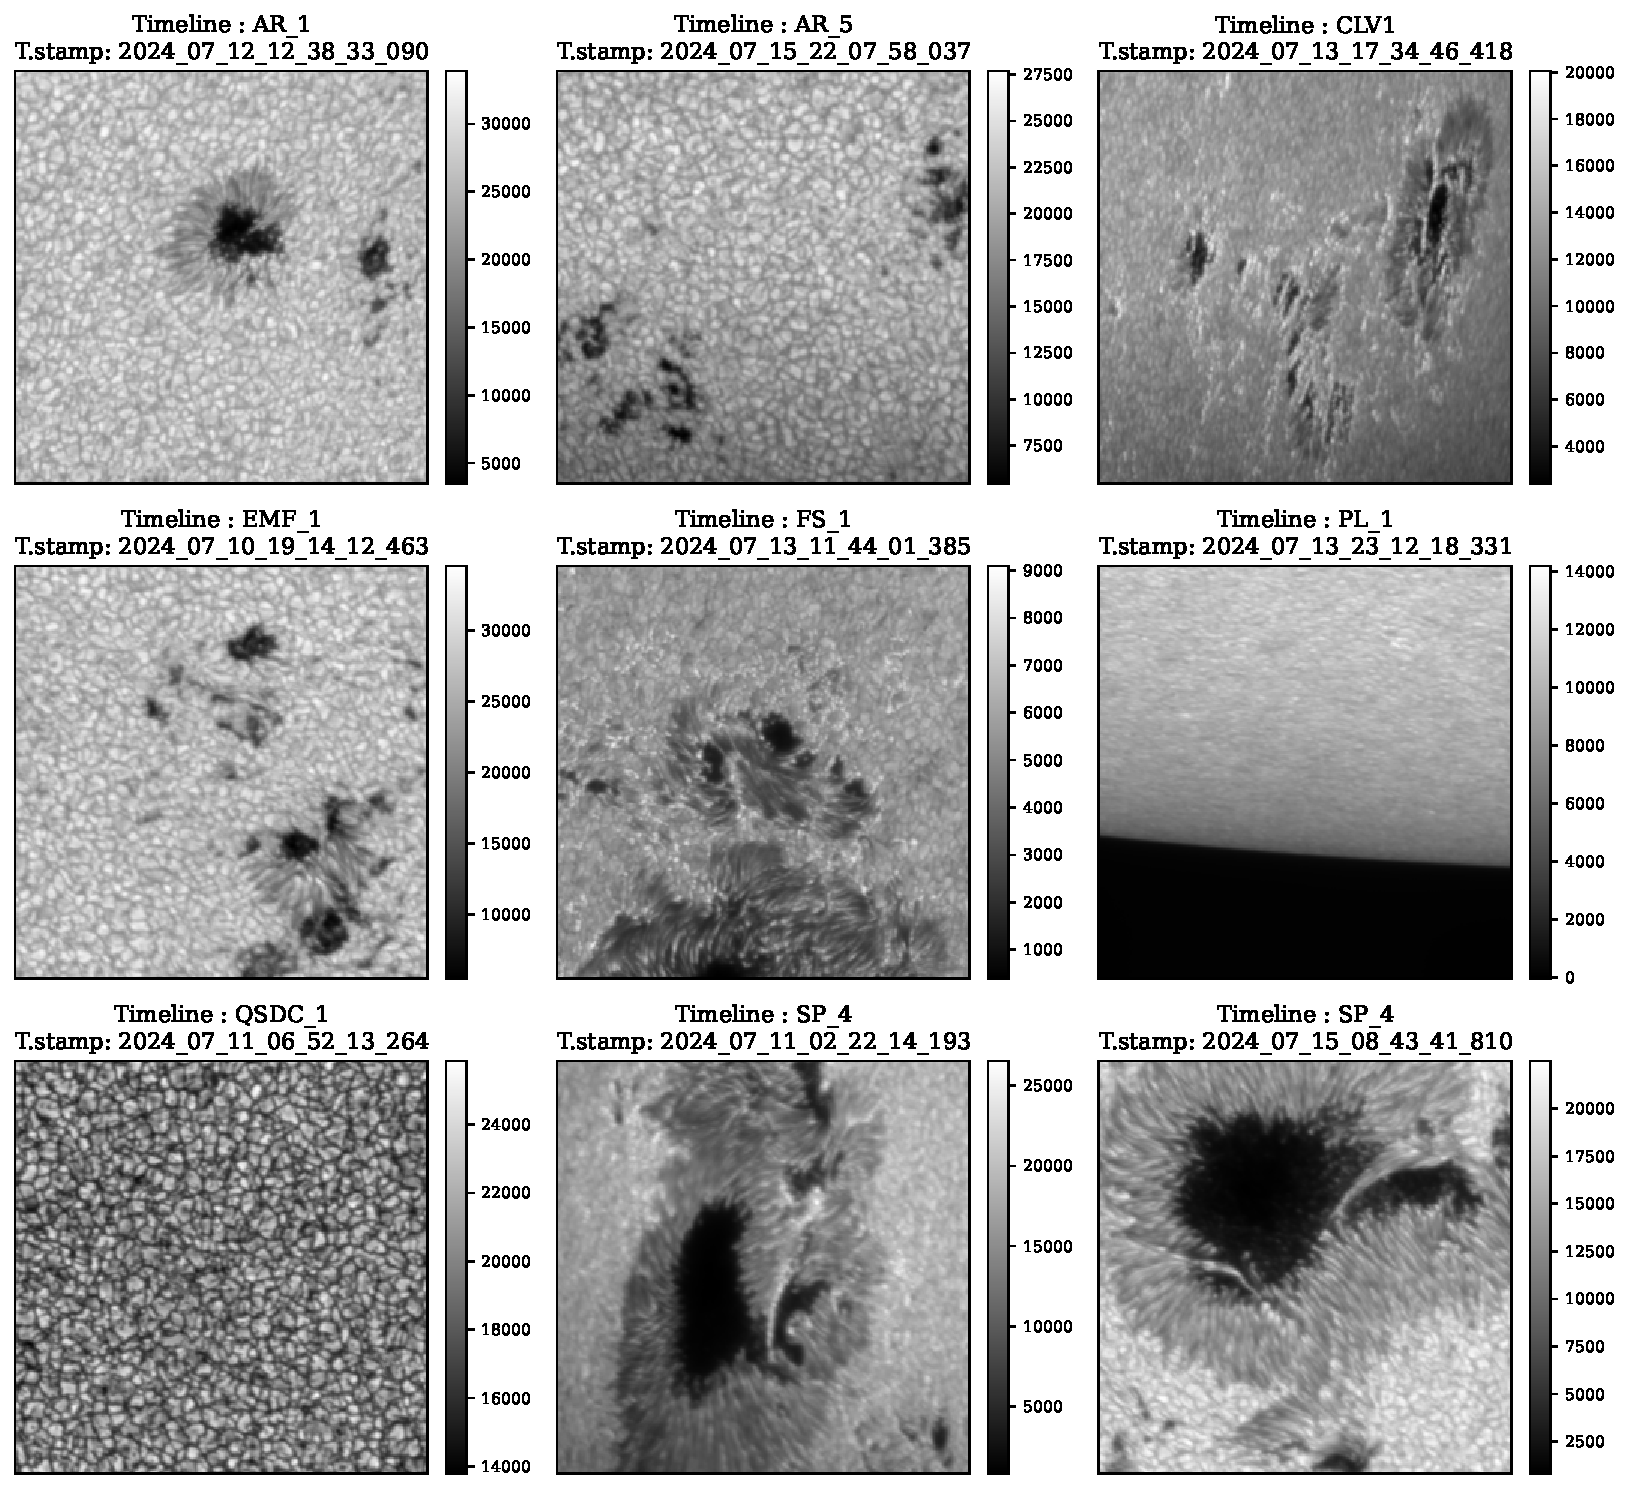
\includegraphics[width=\textwidth]{figures/Pipeline/timelines_Examples.pdf}
  \caption[Timelines mosaic.]{
    Continuum images of the first modulation of the first observation mode from different timelines. The timestamp provided corresponds to the first image of the observation mode. The colorbar is given in counts. All images have been dark-current corrected and flat-fielded. A single flat-field has been employed for all images, instead of the corresponding flat-field for each observation, resulting in some images displaying some intensity gradient.} 
    \label{fig_pipeline: timeline_examples}
\end{figure}

The timelines of the Sunrise III mission can be grouped in the following blocks: 

\begin{itemize}
  \Myitem Quiet Sun observations at disk center (QSDC): focused in regions near the solar disk center that are free from significant solar activity. These timelines typically involve long series of observations aimed at studying the small-scale structure and magnetic flux evolution in the quiet Sun. 
  
  There are four distinct timelines in this category: three standard timelines, which employ the nominal observing modes, and a high-cadence version, the QSDC{\_}HC timeline. The latter employs a modified version of the standard observation modes, where a single wavelength without modulation is recorded at +8 pm of the Fe I 525.02 nm spectral line core, with a temporal cadence of approximately one second. Additionally, it includes a modified version of observing mode 3, featuring fewer accumulations to improve temporal cadence to approximately seven seconds. These high-cadence observations are critical to study the wave propagation throughout the solar surface (see \citealt{acoustic-waves} or \citealt{acoustic-waves-2}).    
  \Myitem Sunspot observations (SP) are specifically designed to study sunspots. There are four different timelines for this purpose. Some of these are short programs used to track the same sunspot over multiple days, with the goal of studying the evolution and decay of the sunspot. Others are more extensive programs aimed at examining, in greater detail, the magnetic activity of sunspots and their penumbral structures.
  \Myitem Polar observations (PL) target the region close to the limb in both poles of the Sun. These areas are of special interest due to their distinct magnetic behavior compared to the disk center. Additionally, these regions provide the opportunity to measure faint signals outside the main solar disk, such as spicules in the lower chromosphere, observed outside the continuum disk in the magnesium line. Two different instances of these timelines were run in the observation campaign which differ by the target spectral lines, and targeted both poles. 
  \Myitem East and West limb (EW) observations are designed to target the equatorial regions of the solar limb. In addition to exhibiting magnetic structures distinctly different from those observed at the poles, the reason for having a separate timeline from the PL timelines lies in the orientation and technical constraints related to SCIP and SUSI's slits. In these EW observations, the spectrometer slits are aligned parallel to the limb, contrasting with the PL timelines, where the slit is positioned perpendicular to the limb.
  \Myitem Active regions (AR) observations are designed to study areas exhibiting solar activity, excluding those specifically focused on the sunspot programs. These observations typically consist of two-hour series, employing the standard combination of the iron 525.02 nm and magnesium lines, using modes 2.02 and 1, which represent the most common observation block for TuMag. Although five different AR timelines were planned for the Sunrise campaign, only three were executed.
  \Myitem Emergence flux (EMF) programs are specifically designed to study active regions that exhibit a large flux emergence. For TuMag, the observation blocks are shared with those of a the AR programs, namely, the combination of mode 1 and 2.02 for series of around 2 hours. 
  \Myitem Full spectral scan (FS) observations are primarily designed for SUSI, where the instrument scans all available wavelength ranges to produce an atlas of the solar spectrum in the near ultraviolet. These scans are intended to be carried out in both quiet Sun and active regions. For TuMag, FS observations consist in long series focusing on the iron spectral line in quiet Sun regions; while in active regions, they include a combination of iron and magnesium observations.
  \Myitem The flares programs (FL) were designedfor flaring regions as targets of opportunity. These programs were intended to be activated only when an active region showed signs of flaring. For TuMag, the observations during these programs consist in the standard combination of iron 525.02 nm and magnesium spectral lines.
  \Myitem Center-to-limb variation (CLV) observations were intended to target regions of the solar disk characterized by $\mu$ values that had not been previously observed. The parameter $\mu$, defined as the cosine of the angle between the surface normal and the observer's line of sight, serves as a useful indicator of a region's proximity to the disk center. Specifically, $\mu$ ranges from 1 at the disk center to 0 at the limb. Conducting CLV observations at previously unmeasured $\mu$ values enables us to capture data from different regions across the disk, facilitating studies of how observational features vary with their position on the disk. 
\end{itemize}

During the Sunrise III observation campaign, 38 timelines were run, including calibration timelines in addition to the scientific programs presented here. Some examples of the different targets employed during the campaign are shown in fig. \ref{fig_pipeline: timeline_examples}.  A detailed record of TuMag's observations can be found online both in the pipeline repository and in TuMag's official data website\footnote{\url{https://www.uv.es/jublanro/tumag_data_test.html}}.  

\section{Pipeline}

\begin{figure}[t]
  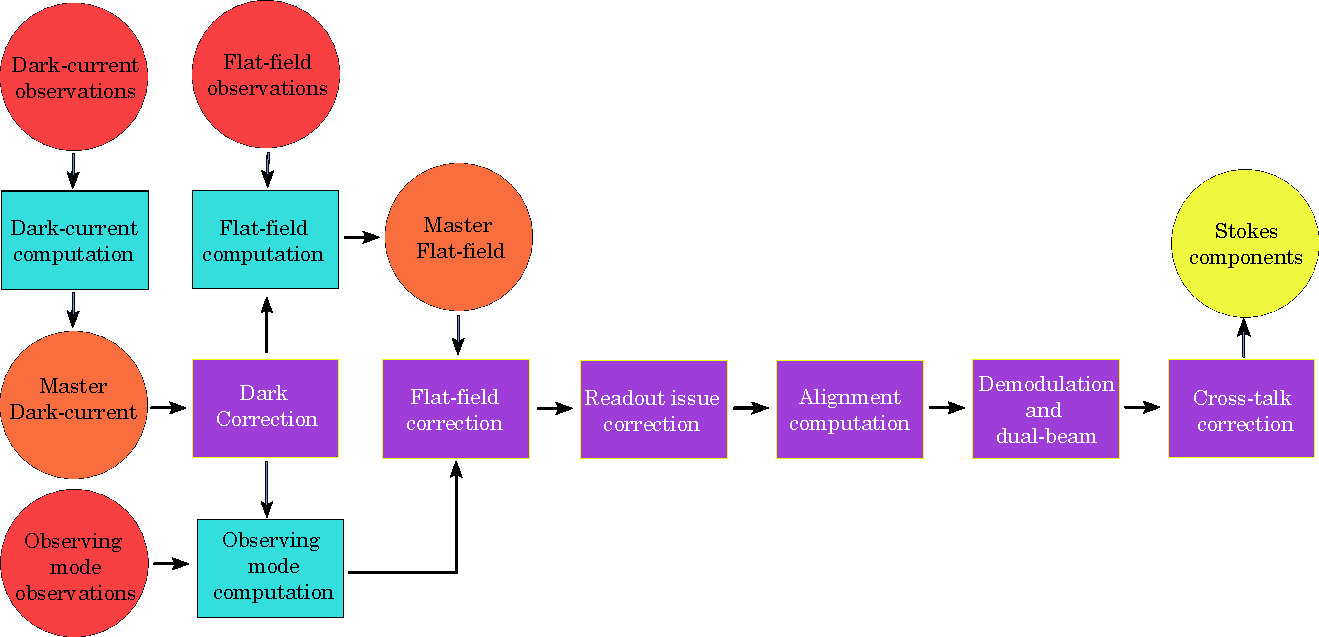
\includegraphics[width=\textwidth]{figures/Pipeline/pipeline_diagram.pdf}
  \caption[Reduction pipeline block diagram.]{
    Block diagram of the standard reduction process: Blue boxes represent image processing steps, and purple boxes the main reduction computations. Red circles represent raw observations, orange circles represent calibration products generated during the reduction, and finally, the yellow circle represents the final product, the Stokes components. }
    \label{fig_pipeline: block_diagram}
\end{figure}

Before data can be employed for scientific purposes, it has to undergo a process where all the instrumental and spurious effects are removed. This process, usually referred to as data reduction, has to be specifically designed for each instrument, as the particular properties of the instrument come into play. Being a spectropolarimeter, TuMag's data reduction pipeline must, in addition to removing the instrumental artifacts, compute the Stokes components of the incoming light.

In this section we introduce the software that has been developed for TuMag's data processing. Due to the proximity of the data's arrival to the end of this thesis, its important to note that the data reduction is still under development, with some calibration steps still undeveloped. In the following, we present the current status of the pipeline, along with a few examples of the results. The pipeline is publicly available in a GitHub repository\footnote{\url{https://github.com/PabloSGN/TuMags_Reduction_Pipeline}}.  

\subsection{Standard data reduction process}

The specific steps that have to be applied to a particular observation depend on the observation mode, and scientific aim of the observation, as different observations  may require additional steps prior to the scientific exploitation. However, most data must go through a common set of steps, typically consisting of the following (see also fig.~\ref{fig_pipeline: block_diagram}):

\begin{enumerate}
  \item Dark current computation. 
  \item Flat-fielding computation (dark-current corrected).
  \item Dark-current correction to observing mode images. 
  \item Flat-field correction to observing mode images (dark-current corrected).
  \item Correction of camera 2 readout issue.
  \item Image alignment between modulations and cameras. 
  \item Demodulation. 
  \item Cross-talk correction and cameras combination.
\end{enumerate}

The data reduction process begins with the dark-current processing, which involves averaging all individual dark frames within a specific set to generate a single dark-current frame per camera. This dark current is then subtracted from all images used in the reduction, including flat-fields, scientific observations, and any other calibration observation, after rescaling the dark-current to the appropriate number of accumulations.

The second step is the flat-field computation. These observations, as previously mentioned, are a modified version of the nominal mode with an increased $\lambda_{\text{rep}}$ and are repeated $N_{\text{rep}}$ times. The processing involves averaging all images taken at a specific wavelength for the same modulation, after applying the dark-current correction to every frame. Thus, $\lambda_{\text{rep}} \times N_{\text{rep}}$ images are averaged to produce a single flat-field frame. To maintain spectral line information, each flat-field frame is normalized to its mean value, as flat-fields taken at the line core have lower intensity than those in the continuum. The goal is to correct intensity variations within a single frame without altering relative intensities across different spectral points.

Having computed the dark-current and the flat-fields, the scientific observations can be corrected by subtracting the dark-current and dividing the resulting image by the flat-field of the corresponding wavelength and modulation. 

\begin{figure}
  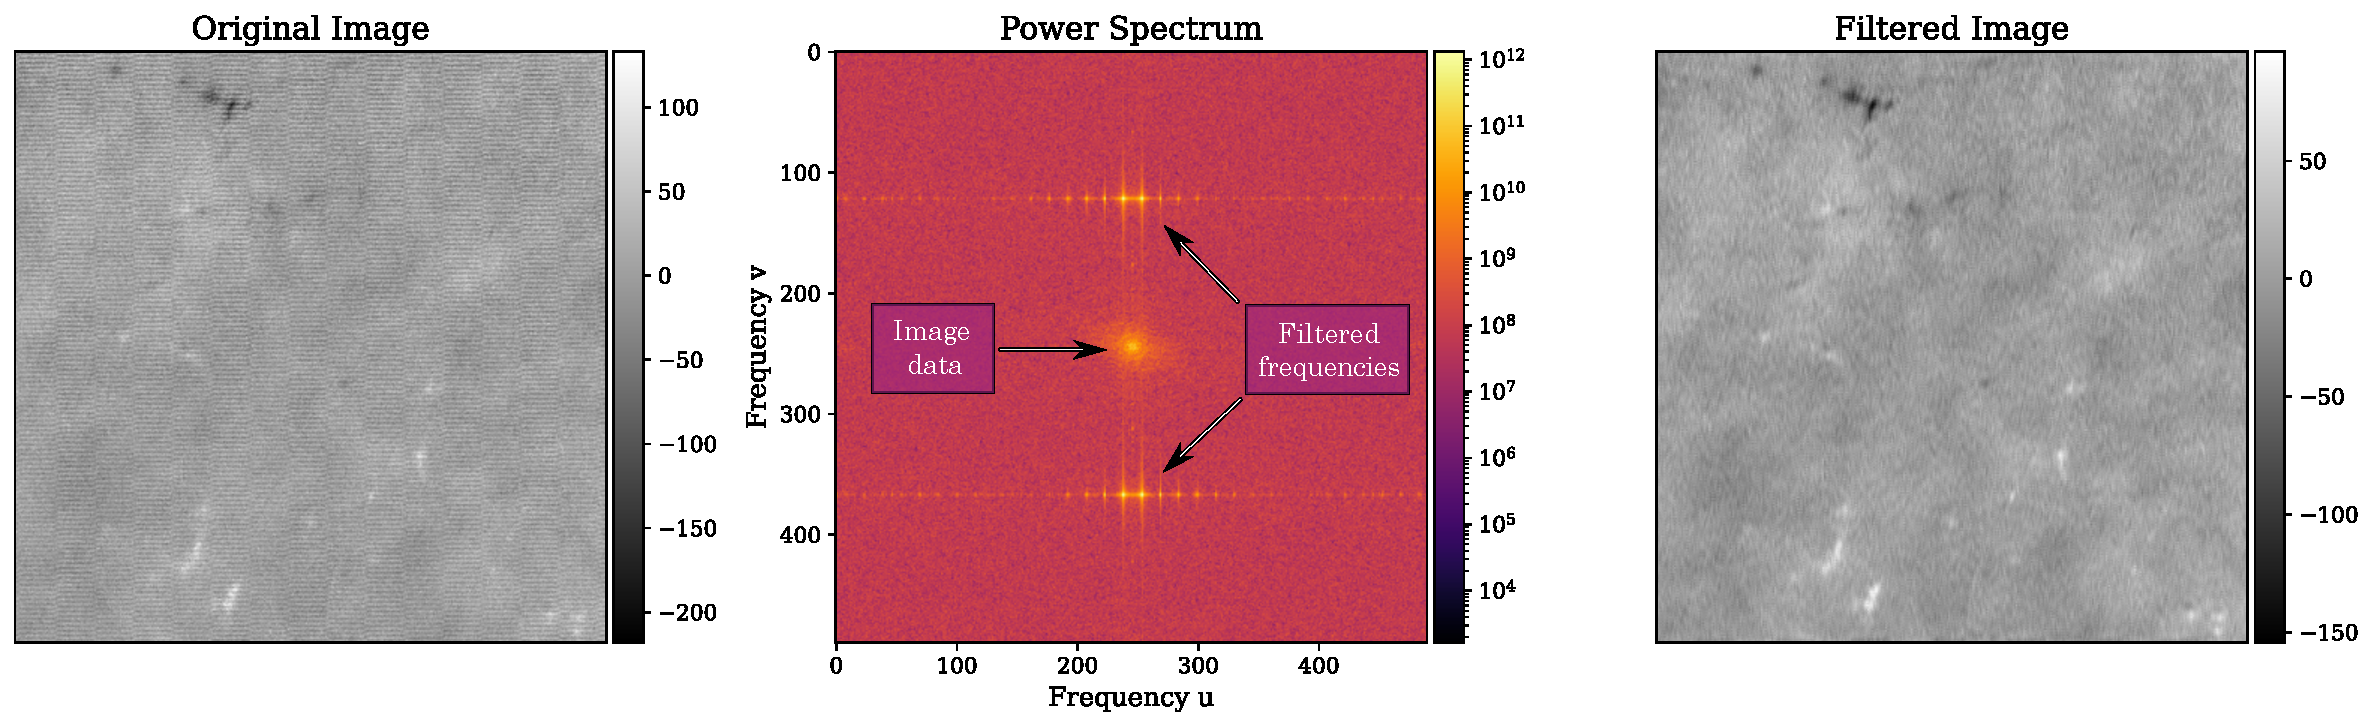
\includegraphics[width=\textwidth]{figures/Pipeline/readout_problem.pdf}
  \caption[Readout pattern filtering]{Left: Uncorrected Stokes U map in the magnesium wing of a quiet Sun observations. Center: Power spectrum of the stokes map showcasing the spatial frequencies of the pattern created due to the readout malfunction. Right: Same map as on the left with the frequencies of the readout pattern filtered out.}
    \label{fig_pipeline: readout}
\end{figure}

In addition to dark-current and flat-field corrections, an additional adjustment is required before proceeding with further computations. During operations, the second camera developed a readout issue that was not present during calibrations. This malfunction introduces a recurring spurious pattern in all frames taken by this camera (see the left panel of Figure \ref{fig_pipeline: readout}). Fortunately, this structure is consistent throughout all measurements and is characterized by a repetitive pattern whose intrinsic spatial frequencies can be identified in the power spectrum (see central panel of Fig.~\ref{fig_pipeline: readout}), allowing it to be effectively filtered out by manually setting the corresponding frequencies to zero in the fourier domain before reconstructing the image from their power spectrum. The result of this procedure is shown in the right panel of Figure \ref{fig_pipeline: readout}.  


Before computing the Stokes components, the images from different cameras and modulations must be accurately aligned, as they will be combined during demodulation. Any misalignment of the solar structures in the images results in the apparition of spurious polarization signals. The alignement process is carried sequentially: first, images belonging to the first camera of different modulations are aligned between them; then, the images captured by the second camera are aligned with respect to the images of the corresponding modulation of the first. This alignment is performed with subpixel accuracy using the method described in \cite{alineamiento}, which calculates the alignment via a two-dimensional cross-correlation in the Fourier domain.

The Stokes parameters are then computed by applying the demodulation matrix to the aligned and corrected modulations. If the polarimetric response is consistent across the FoV, an average demodulation matrix can be applied uniformly. However, if the system exhibits significant variation across the FoV, a two-dimensional demodulation approach where a unique matrix is assigned to each pixel is required, as large deviations from ideal demodulation are challenging to correct. TuMag's pipeline incorporates both approaches, allowing selection based on the demodulation performance. 

After demodulation, data from both cameras are combined into a single map for each Stokes component and wavelength. This is done by adding the Stokes maps from both cameras while normalizing for intensity differences. Combining images from different cameras measuring orthogonal polarization states effectively removes most jitter-induced cross-talk.

\begin{figure}
  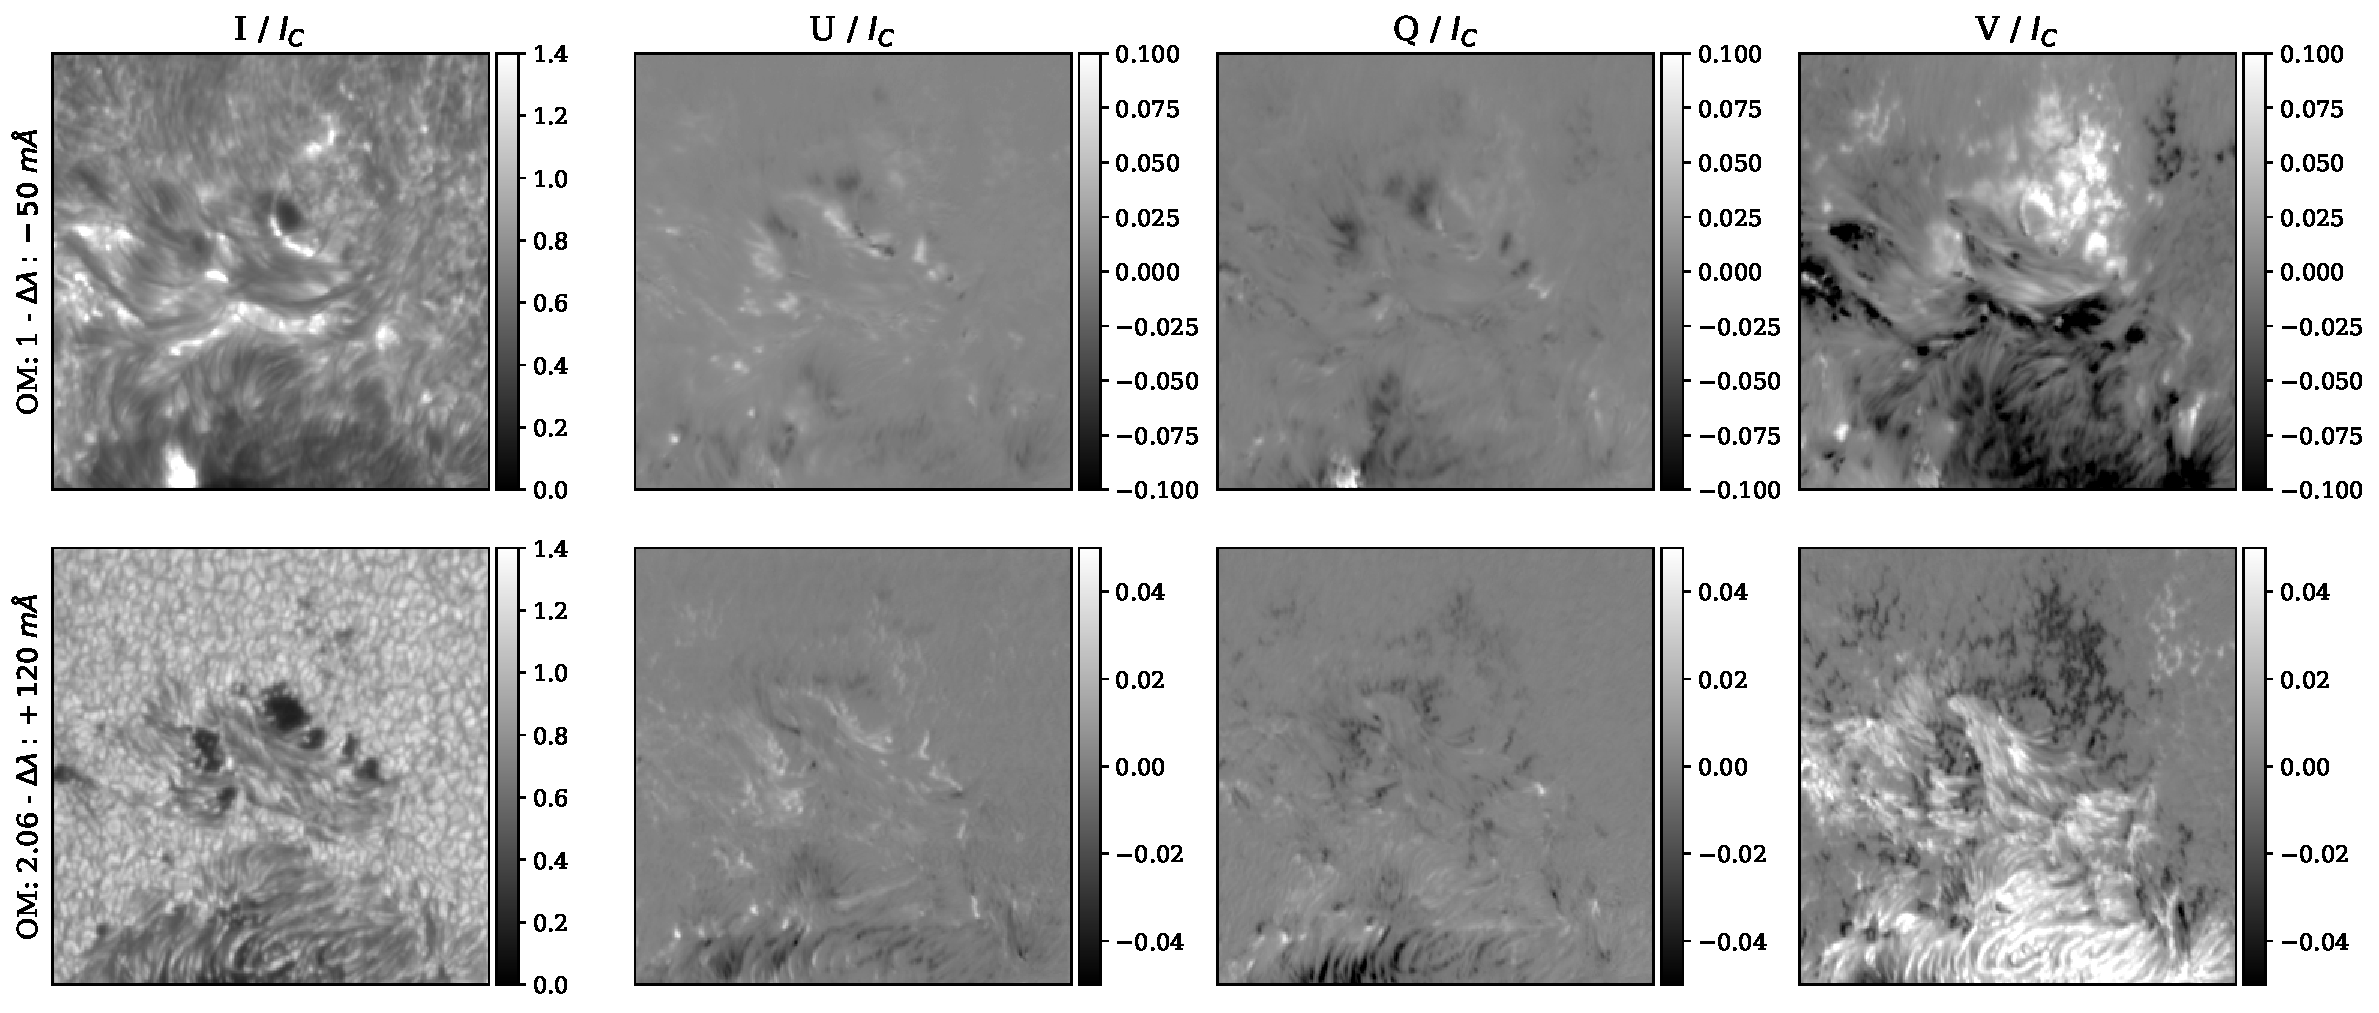
\includegraphics[width=\textwidth]{figures/Pipeline/Example_demodulation.pdf}
  \caption[Stokes maps for magnesium and iron.]{Stokes maps in magnesium (top row) and iron 525.06 nm (bottom row) lines wings, measured at -50 m\r{A} and +120 m\r{A} from the line core, respectively. No cross-talk correction has been applied. The observation corresponds to a FS timeline ran in a flaring active region. Timestamp of the first observation mode (mode 1) : 2024/07/13 12:28:00.  }
    \label{fig_pipeline: demodulated_data}
\end{figure}

Figure \ref{fig_pipeline: demodulated_data} shows an example of the demodulated stokes maps for observing mode 1 (magnesium) and 2.06 (iron 525.06 nm) at the wings of the spectral line. The intensity map in the magnesium shows the beginning of a flare around the central sunspot. 

\begin{figure}
  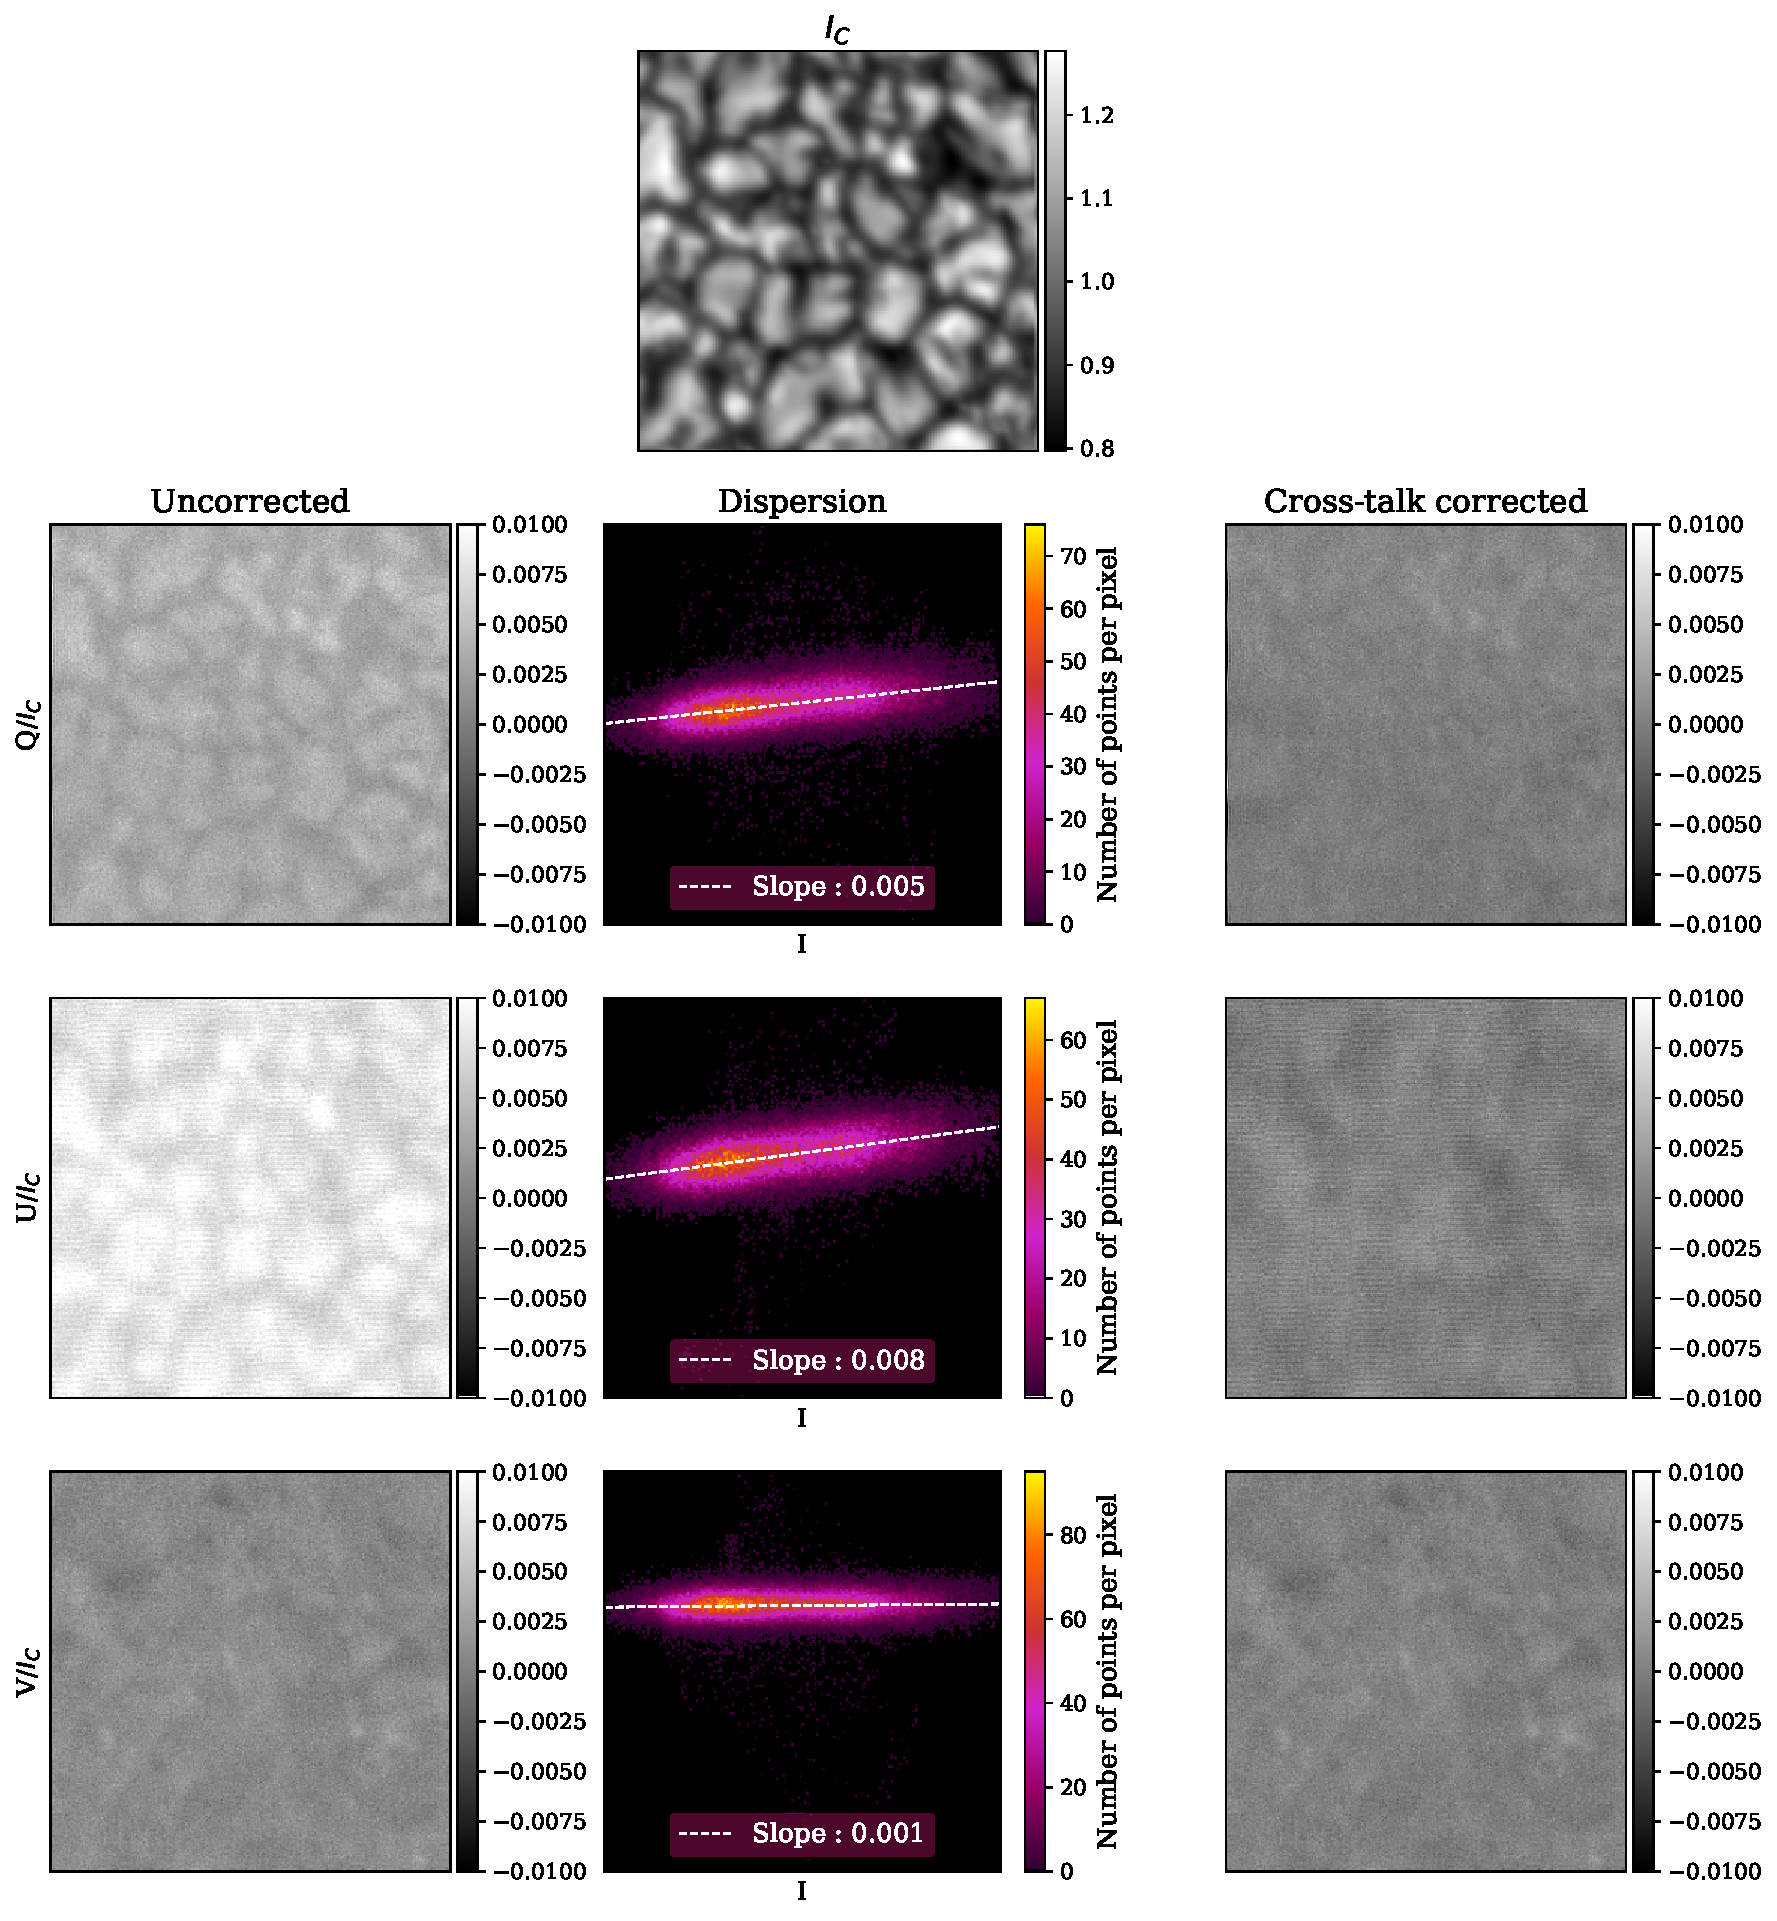
\includegraphics[width=\textwidth]{figures/Pipeline/xtalk_example.pdf}
  \caption[Cross-talk correction.]{Example of a cross-talk correction in a small region of the FoV. Each row shows a different stokes parameter. The left column shows quiet Sun stokes maps after demodulation, the central column shows the dispersion between the intensity and the corresponding stokes parameter, and the right column shows the corrected maps. In this data set, the readout problem has not been assessed and is clearly discernible in Stokes U.}
    \label{fig_pipeline: xtalk}
\end{figure}


Due to minor pixel-to-pixel variations when using the average demodulation matrix or residual instrumental artifacts not corrected by flat-fielding, the demodulation process is often imperfect. These imperfections result in contaminated Stokes components, where information from one component appears in others, typically with leakage from Stokes I into Q, U, and/or V. However, if the demodulation matrix closely approximates the ideal matrix, this contamination, known as cross-talk, can be corrected.

Cross-talk contamination between Stokes I and any other given Stokes component can be assessed in regions of the FoV without solar structure, using the continuum. In these regions, linear polarization signals should be almost absent. One method to quantify cross-talk from one component ($I$) to another ($S_{\text{cont}}$) involves fitting a line to the dispersion map created by plotting one component against the other. The slope of this line indicates the cross-talk level, as no correlation should exist in quiet Sun areas \citep{crosstalk-manolo}. Once this relationship is established and the cross-talk intensity is measured, the correction is applied by removing this linear trend from the data:

\begin{equation}
  S_{\text{corr}} = S_{\text{cont}} - I a + b,
\end{equation}
where the relation between the stokes component $I$ and $S_{\text{cont}}$ has been fitted to the line: $S_{\text{cont}} =  I a + b$.

Figure \ref{fig_pipeline: xtalk} shows an example of a cross-talk correction in a small region of the FoV in the continuum of a quiet Sun observation. The granulation structure is clearly visible in Q and U before the correction. The central panel shows the dispersion between the corresponding Stokes component and the intensity, along with the fitted relation. In the case of Q and U, the relation is clearly stronger than in V, where the slope is almost 0. The right columns shows the result of the correction, with Q and U without the majority of influence of the intensity, although some traces can be found. Nevertheless, the cross-talk before the correction is below the 1\%, and thus, the polarimetric sensitivity is larger than $10^{-3}$.
\subsection{Extra calibration blocks}

As previously presented, TuMag observations include a series of calibrating observing modes that are not employed in the standard reduction process, namely, polarizers observations, both the linear polarizer and the micropolarizers set, the pinhole observations, prefilter scans, or PD. These sets of calibrations are meant to be processed separately to aid with the data reduction in observing modes that require it.

The processing of these steps is still in an early stage, and are expected to be fully developed in the following months. Nonetheless, we will now outline the purpose of these observations and their intended role in the reduction process.
\subsubsection{Image reconstruction}

\begin{figure}[h]
  \begin{minipage}[c]{0.67\textwidth}
    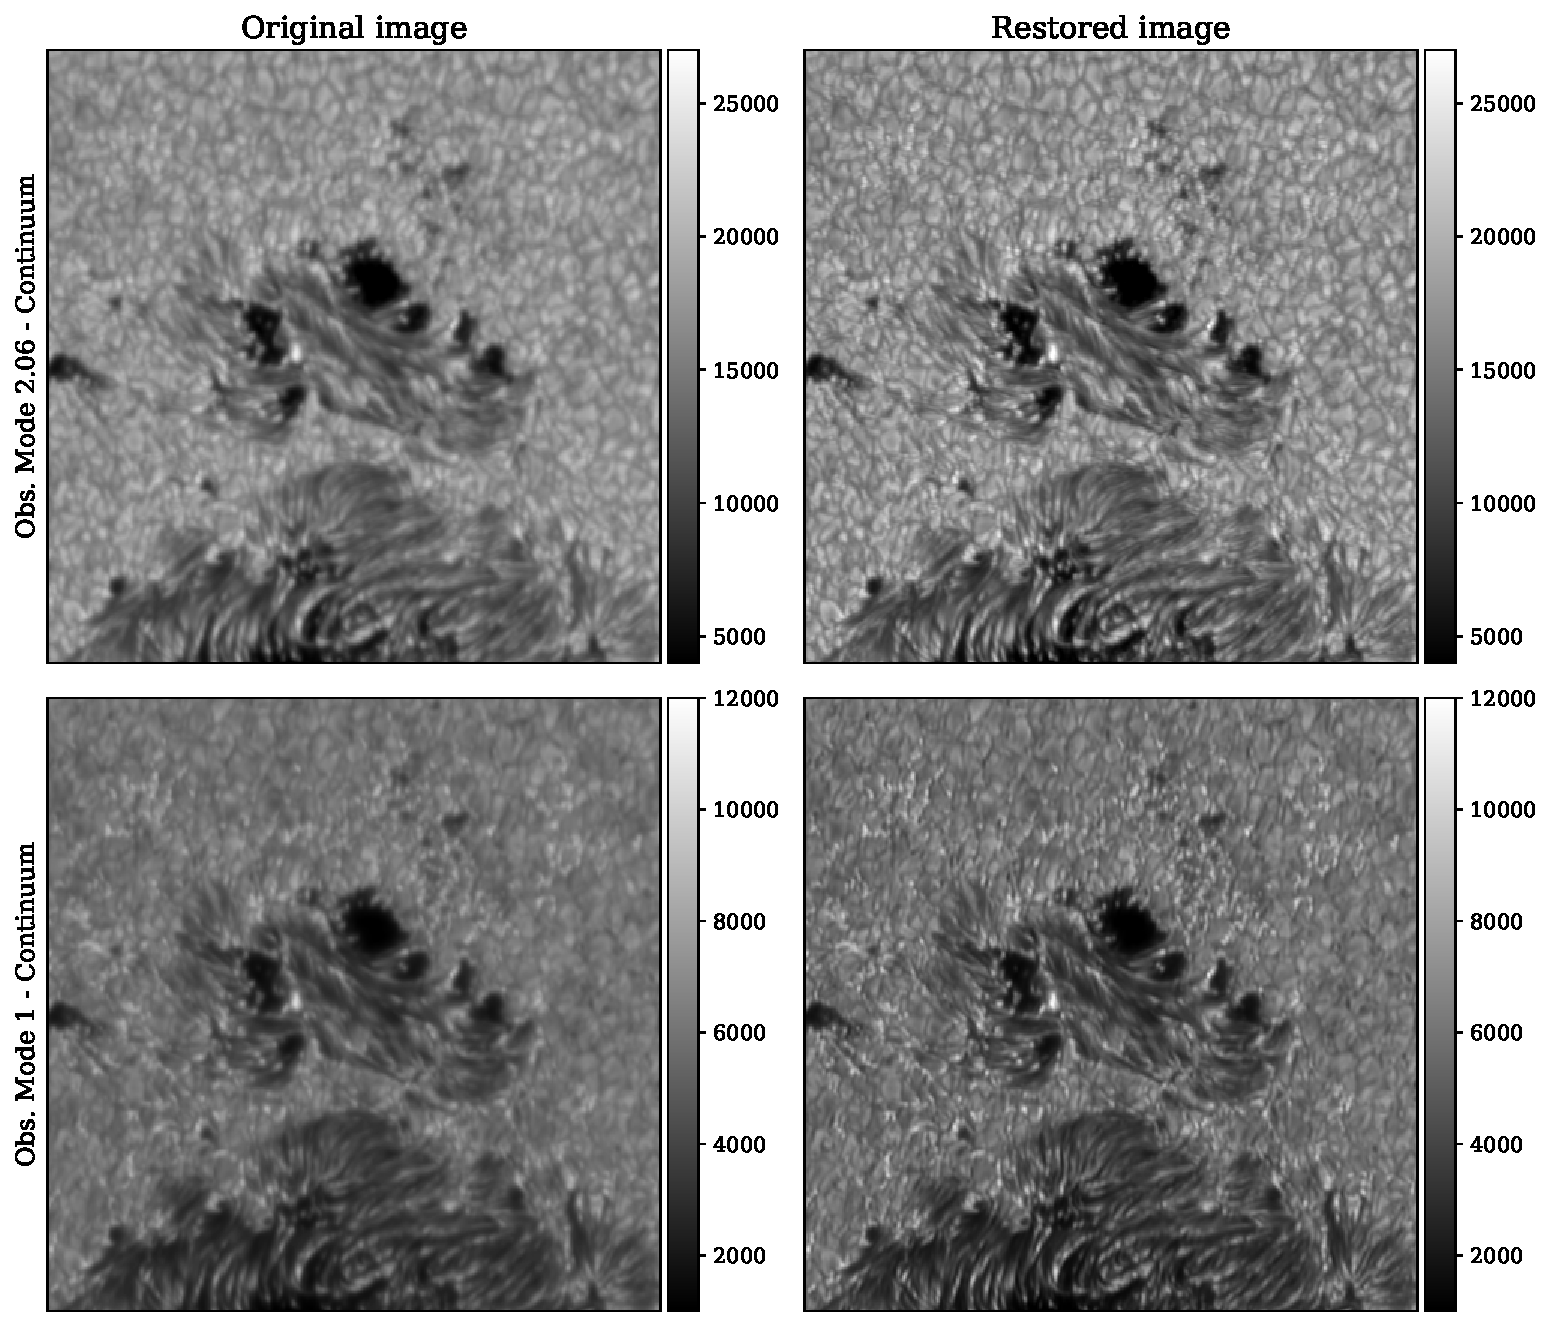
\includegraphics[width=\textwidth]{figures/Pipeline/Image_restoration.pdf}
  \end{minipage}\hfill
  \begin{minipage}[c]{0.29\textwidth}
    \caption[Image reconstruction.]{
     Example of image reconstruction in the FS timeline for both the 517 nm (Obs. Mode 1) and 525.06 nm (Obs. Mode 2.06) pre-filters. The data set for the PD measurements was taken on the 13$^{th}$ at 11:42 UT. The timestamp of the first image of the first observation mode is: 2024/07/13 12:28:00 UT. PD computation made by F.J. Bailén.
     \label{fig_pipeline:  image_restoration}} 
  \end{minipage}
\end{figure}

Image reconstruction is, in truth, one of the steps in the main data pipeline and will eventually be implemented as an additional step applicable to all datasets to maximize TuMag spatial resolution potential. However, it has been separated in this description because it is not yet fully developed and ready for automatic processing across all datasets.

The image reconstruction technique consists in deconvolving the PSF of the instrument from the data through a Wiener-Helstorm filter (see sec. \ref{sec: intro-imaging}). PD measurements (see sec. \ref{susec: PD_measurements}) are employed to derive the PSF though the determination of the Zernike parameters that describe the WFE. These PD measurements are taken before and after scientific observations to ensure the aplicability of the reconstruction throughout the whole data series.

Figure \ref{fig_pipeline:  image_restoration} shows an example of such a reconstruction, for the 517 nm and 525.06 prefilters. The reconstruction employs the closest PD measurement dataset to the observation and 21 Zernikes for the PSF determination.   

\subsubsection{On-flight polarimetric calibration}
\begin{figure}[t]
  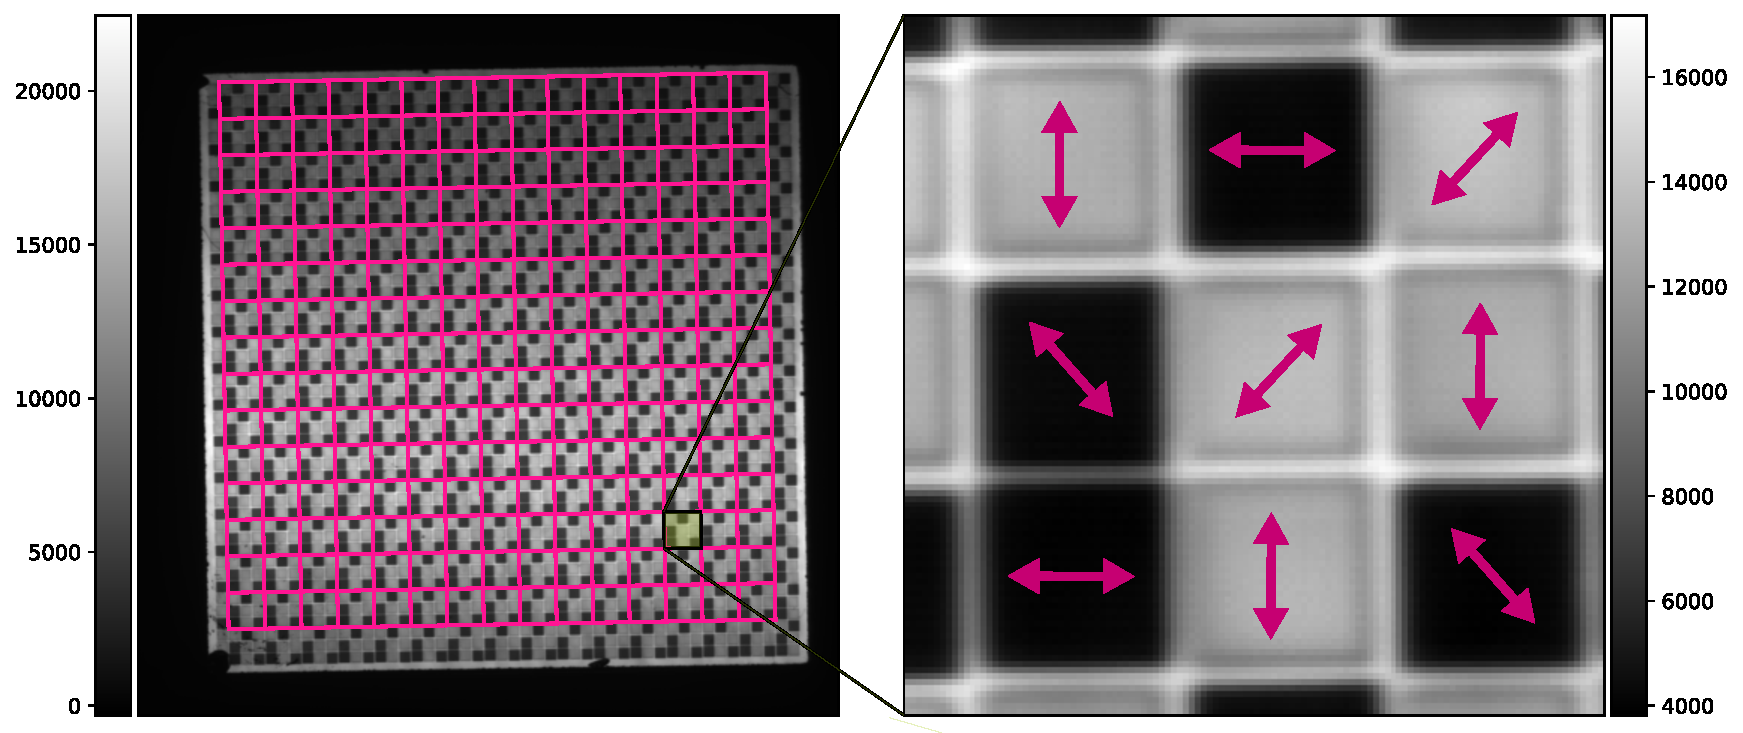
\includegraphics[width=\textwidth]{figures/Pipeline/Micrpols_edit.pdf}
  \caption[Micropolarizer observations.]{
   Micropolarizer observation with the boundaries of the array of linear polarizers overplotted. The right panel shows the orientation of the linear polarizers that compose each array.}
    \label{fig_pipeline: micropols_calib}
\end{figure}

The presence of cross-talk in the observations can arise from deviations of the instrument modulation with respect to the modulation derived during on-ground calibrations. In such cases, the demodulation matrix used in the pipeline diverges from the ideal matrix, resulting in a suboptimal demodulation process. However, TuMag is equipped with both linear polarizer and micropolarizer targets to evaluate the demodulation schemes.

Both polarizer targets can be utilized to assess the level of cross-talk in the observations. When a linear polarizer is placed in front of the instrument, no circular polarization should be inferred after proper processing and demodulation. Any residual circular polarization would indicate the level of cross-talk from Stokes I to Stokes V. Similarly, knowing the polarizer's orientation relative to the instrument, it is possible to quantify cross-talk between Stokes Q and U, something that is not easily achievable with regular observations. These calibrations are still ongoing but will help us enhance the instrument's polarimetric accuracy beyond the standard cross-talk corrections commonly applied in solar observations. Additionally, the approach includes modifying the modulation matrices themselves, which is a more effective method for maintaining low cross-talk levels.

Micropolarizer observations further allow this assessment to be performed across different regions within the FoV. The micropolarizers are composed of 3 x 3 arrays of small linear polarizers, each oriented in different directions (see Figure \ref{fig_pipeline: micropols_calib}). This setup enables the same evaluation conducted with the linear polarizer to be applied to each individual micropolarizer.


\subsubsection{\label{sect:pipeline_prefilter_scans_fit}On-flight spectral calibration}

One of the most important calibration procedures that is still under development is the on-flight spectral calibration or pre-filter extraction. From both the on-ground calibrations and the spectral scans conducted during flight (see Sect. \ref{ref:spectral_scans}), it is evident that the pre-filters are not perfectly centered, and the measured intensity is affected differently depending on the spectral position. In particular, magnesium line observations are the most affected by this owing to the extended width of the spectral line.

\begin{figure}[t]
  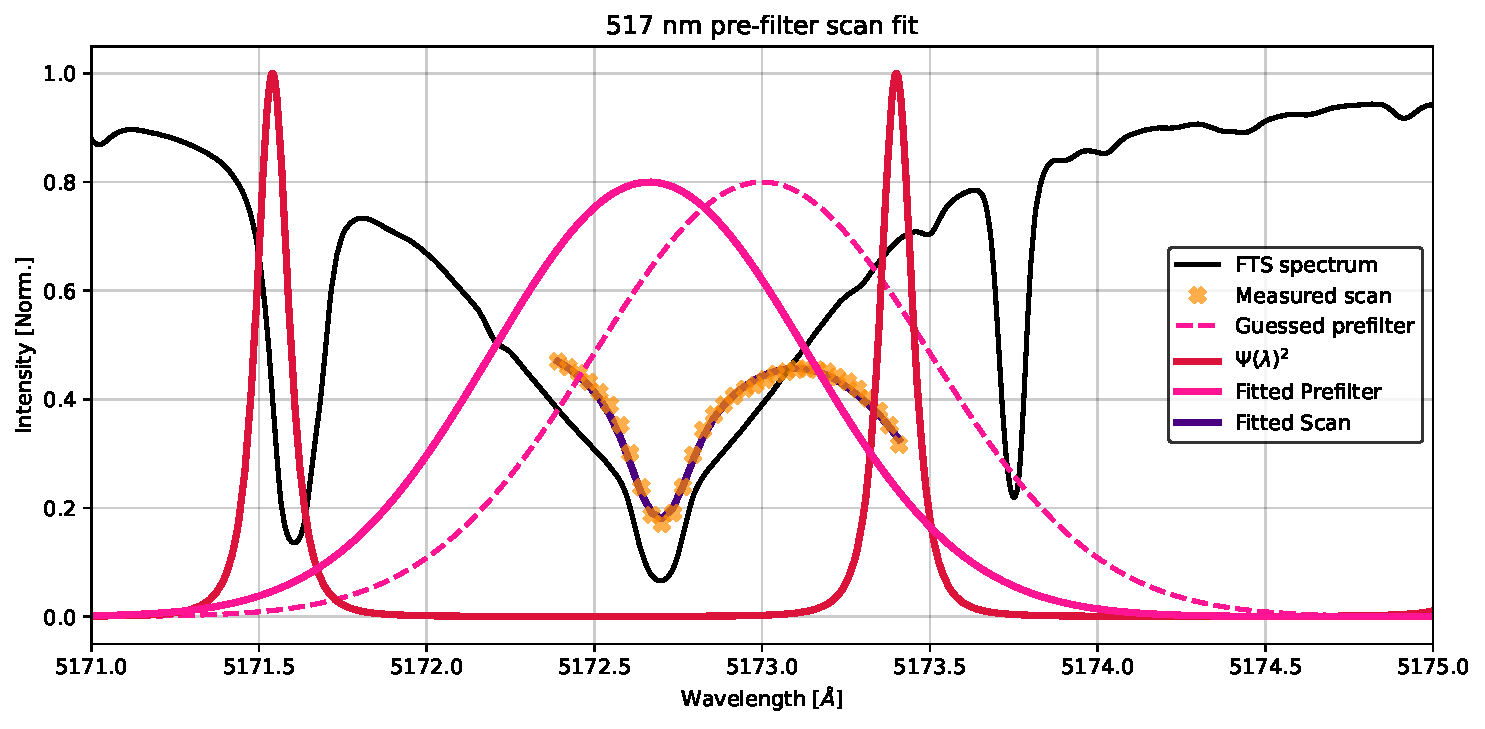
\includegraphics[width=\textwidth]{figures/Pipeline/Prefilterfit.pdf}
  \caption[Prefilter fitting.]{
    Fitting of the 517 nm pre-filter scan recorded on the 10$^\text{th}$ of July at 14:21 UTC during the commisioning phase. The pre-filter measurements (orange crosses) have been normalized to the expected intensity of the spectral line for better comparison. The dark blue line shows the expected scan for the fitted pre-filter (solid pink line) and the etalon transmission profile (red).}
    \label{fig_pipeline: prefilter_fit}
\end{figure}


By analyzing the pre-filter scans—recorded with rich spectral sampling—and using an analytical model of the etalon's transmission profile, we can carefully assess the contributions of both the second order and the pre-filter effects through a fitting procedure. Specifically, we compare the expected intensities for a given pre-filter position and etalon parameter set to the observed intensities. This comparison enables us to fit the pre-filter and/or etalon properties to match the observations.

Figure \ref{fig_pipeline: prefilter_fit} illustrates an example of this analysis for the magnesium pre-filter, where only the width and spectral position of the pre-filter peak transmission were fitted. The results indicate a slight redshift of the pre-filter relative to the line core. While small, this shift allows contamination from the etalon second order, introducing light from the spectral line at $\sim$5171.6 \r{A} into the measurements of the magnesium line right wing. These type of studies enable the correction of pre-filter effects and the quantification of second-order contamination, allowing its removal from the measurements.

These results are preliminary and require enhancements, such as replacing the Gaussian model with the actual pre-filter transmission profile and incorporating a more complex etalon model that includes stray-light contamination. The fitting procedure employs Newton's method, utilizing analytical expressions for the transmission profiles and their derivatives. This method, originally developed for other works, was designed with TuMag applications in mind and will be discussed in detail in the next chapter.
